% Chapter 3

\chapter{Results} % Main chapter title

\label{Results} % For referencing the chapter elsewhere, use \ref{Chapter1} 

\lhead{Chapter 5. \emph{Results}} % This is for the header on each page - perhaps a shortened title





\section{Into The Performace of The Novelty Search Method}


\begin{figure}[ht!]
\centering
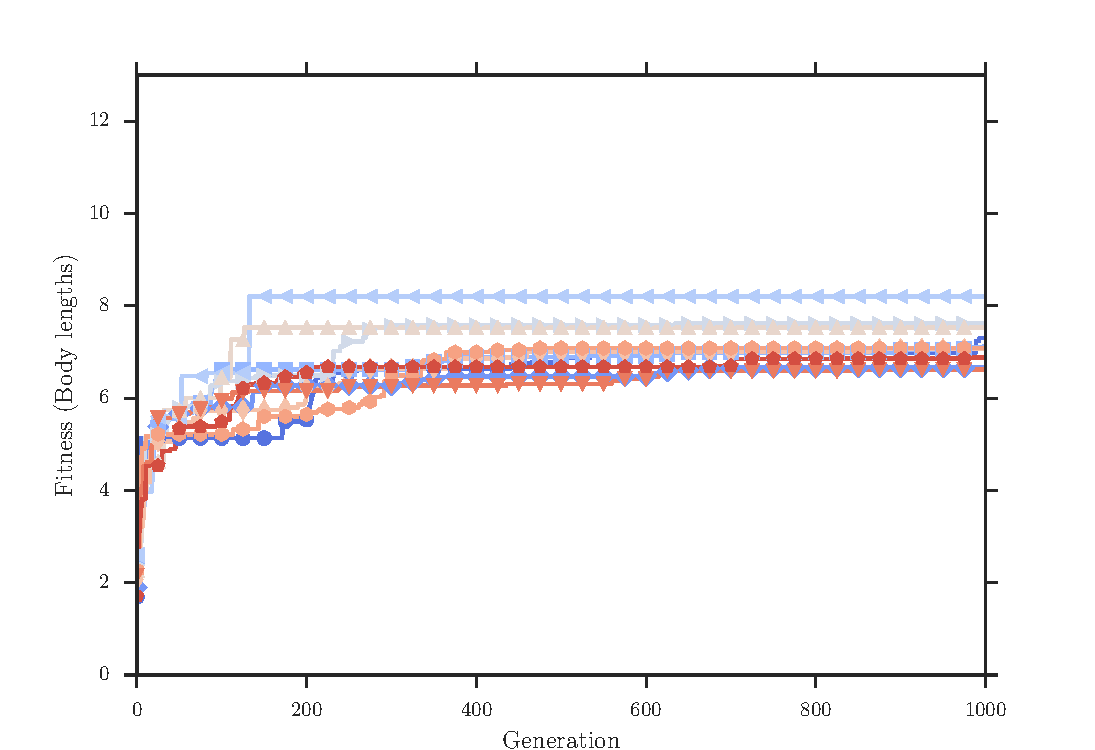
\includegraphics[width=1.0\textwidth]{../Figures/Results/indRunnAvgSize7Fitness.pdf}
\caption{Best fitness so far, average fitness from $10$ individual runs for fitness based search (settings~\ref{Settings3}).}
\label{fig:indRunsAvgSize10Fitness}
\end{figure}

Figure~\ref{fig:indRunsAvgSize10Fitness} shows $10$ independent runs for fitness based search, alongside the mean of these runs' fitness. Following the objective function's gradient fitness based evolution does small step towards better and more optimized individuals from generation to generation. What is more, fitness based evolution often sticks on shapes which then tries to optimize leading the evolution to stop at that local maximum.

\begin{figure}[ht!]
\centering
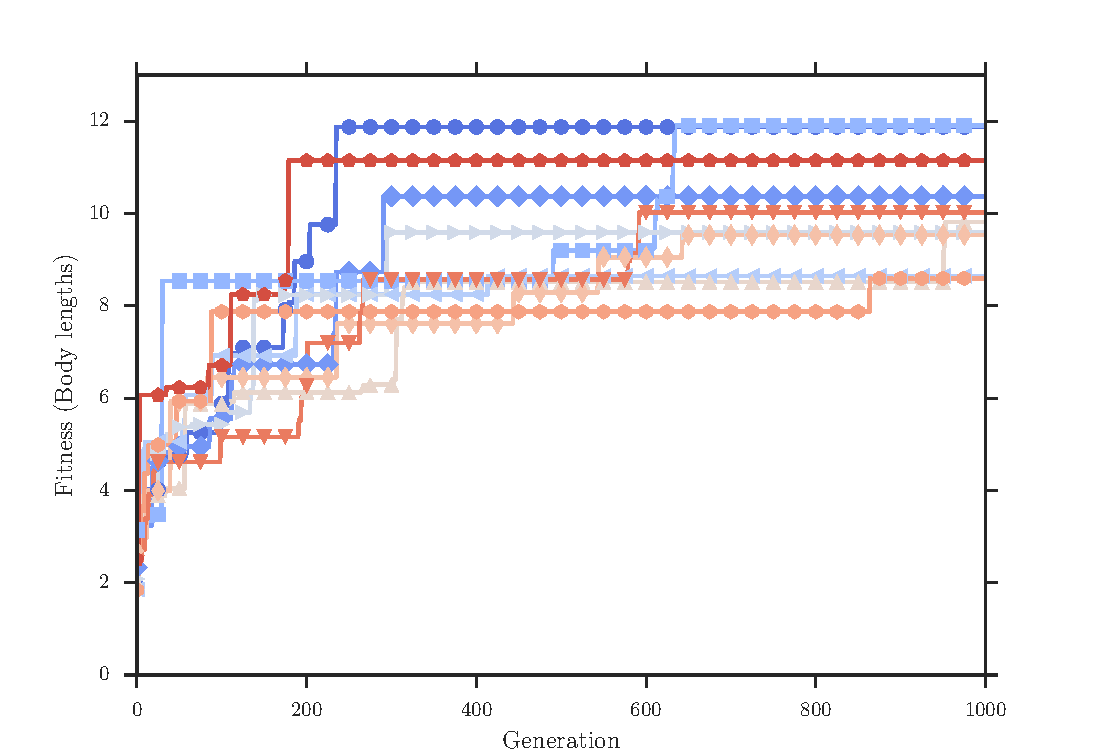
\includegraphics[width=1.0\textwidth]{../Figures/Results/indRunnAvgSize7Novelty.pdf}
\caption{Best fitness so far, average fitness from $10$ individual runs for novelty search (settings~\ref{Settings3}).}
\label{fig:indRunnAvgSize10Novelty}
\end{figure}

Figure~\ref{fig:indRunnAvgSize10Novelty} shows $10$ independent runs for novelty based search, alongside the mean of these runs' fitness. In comparison with the same figure for fitness based search we can see a clear difference. Evolving for novelty means that within the evolution only a novel behavior is rewarded instead of a good behavior or a behavior that leads to the optimization of the objective function. Big steps in the fitness value on all independent runs can be observed which can lead us to a conclusion that fit individuals in respect to the objective function for which novelty search has no information within the evolution process, are not optimized as they could. Initially novel individuals are highly rewarded, these individuals could be very good in respect to the fitness or not, the algorithm does not consider how individuals can be measured in respect to the objective function and does not have any information regarding this either. On the next generation, mutations, crossovers, or even copies of these novel individuals are not going to be highly variant in respect to their genotype's topology from their ancestors, resulting to similar behaviors which are going to be unremarkably rewarded as far as their novelty is concerned. Thus, highly novel individuals are producing less novel children, meaning that these children, even though their fitness is high, will not have the chance to reproduce in the next generations and be improved eventually, as in fitness based evolution.


\begin{figure}[ht!]
\centering
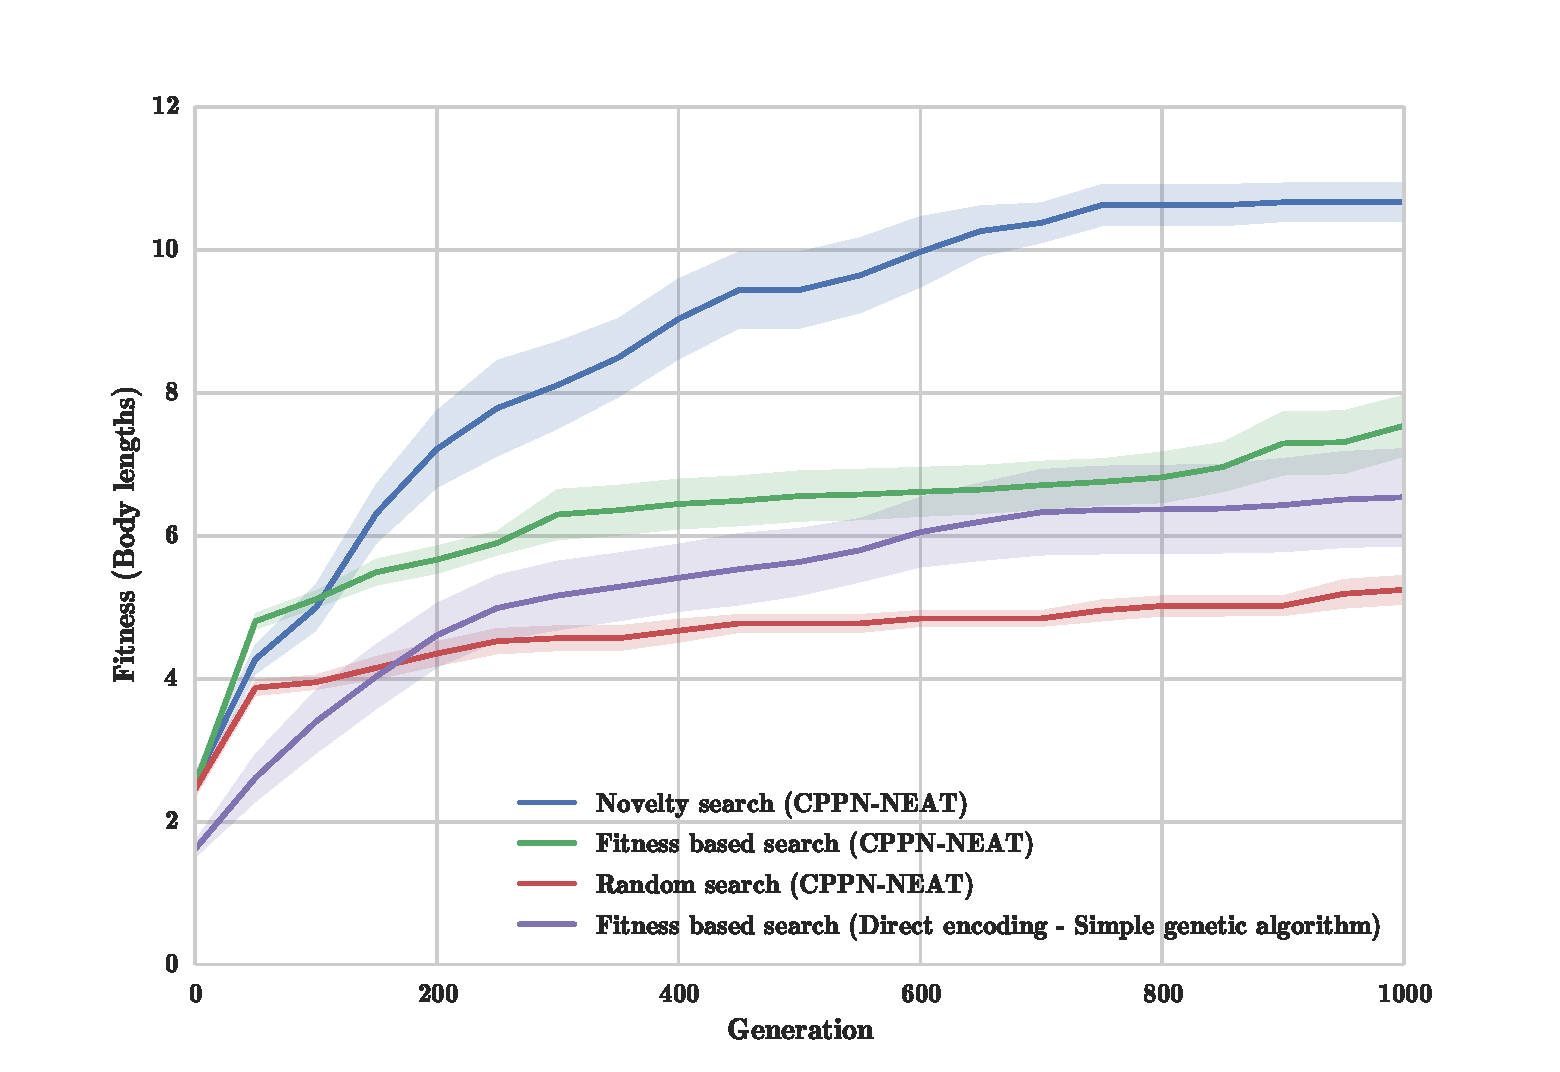
\includegraphics[width=1.0\textwidth]{../Figures/Results/FitNovRandomDirectSize5.pdf}
\caption{Comparison of simple genetic algorithm (direct encoding) against \emph{random} - \emph{fitness} - \emph{novelty} search with generative encoding. Best so far fitness averaged over $10$ runs (settings~\ref{Settings1}).}
\label{fig:FitNovRandomDirectSize5}
\end{figure}

\begin{figure}[ht!]
\centering
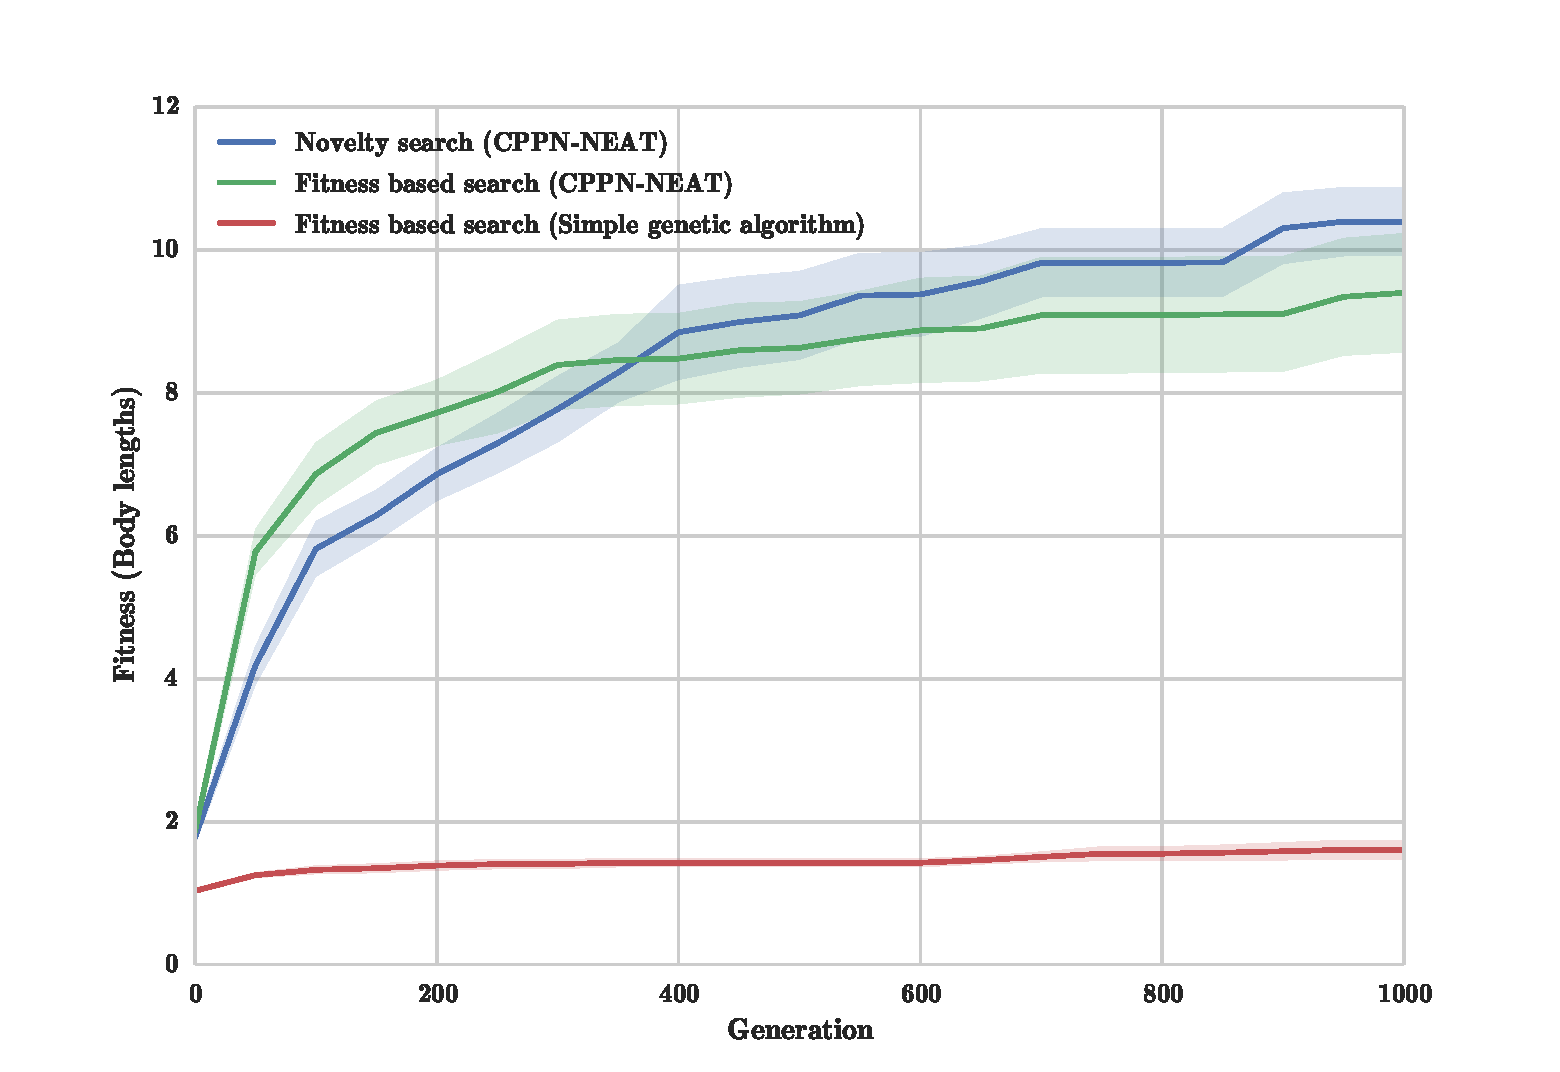
\includegraphics[width=1.0\textwidth]{../Figures/Results/FitvsNovVsDirSize10.pdf}
\caption{Comparison of simple genetic algorithm (direct encoding) against \emph{fitness} - \emph{novelty} search with generative encoding. Best so far fitness averaged over $10$ runs (settings~\ref{Settings2}).}
\label{fig:FitvsNovVsDirSize10}
\end{figure}


To directly compare the performance achieved by novelty search method the same experiment held under two different simulation settings, set side by side with fitness search, random search, and finally a simple genetic algorithm. Notice that the first three methods are referring to a generative encoding (CPPNs) evolved by Hypercube NEAT evolutionary algorithm, while the latter uses a direct encoding scheme. Novelty search to perform the novelty metric computation, makes use of the two dimensional trajectories, which are all normalized so that their centre of mass of the trajectories coordinates meet a specific angle, as well as their starting coordinate is always located in the beginning of both axes. Fitness-based search objective function is the displacement of the soft-robot's center of mass from its initial position in body-lengths. Random evolution with Hypercube NEAT achieved using random selection among generations as well as the mutation power, and the probabilities of adding new links and nodes in the genotypes' CPPNs are all increased, so more complex networks will be evolved during the process of evolution. For direct encoding, the method used is the one explained in Chapter~\ref{Method}. 

The simulation settings used were identical apart from the size of the structures allowed. Figure~\ref{fig:FitNovRandomDirectSize5}, presents the results for the small sized structures ($<5 \times 5 \times 5>$). Notice, the difference between fitness-based search and novelty search methods, novelty evolves structures that superior than any other method does in these settings. At this point, it should be mentioned that in such a small structures locomotion patterns cannot be evolved due to the stability issues of the simulator, and due to the fact that lightweight structures can be bouncy, leading to ball shaped structures capable of achieving large displacement from their initial positions. That being said, we still have to deal with an optimization problem, where local optima and global ones can be found as the number of the possible solutions in this setting, using 4 materials, is $\sim 2,3 \times 10^{87}$, which is lower when all unconnected parts are removed before the simulation. Using the trajectories of the soft-robots novelty search visits optimal solutions that none of the other methods does probably because of local optima (fitness-based search), due to encoding limitations (direct encoding), or random search which approximates novelty search, but with no backtracking (there is no guarantee that random search will visit new behaviors). Direct encoding of the genotype also achieves high performance in relation to random and fitness search something adding importance to the fact that in such small and lightweight structures there is no much gain using generative over direct encoding. 

To eliminate the fact that smaller structures cannot give a proper estimation of a soft structure's displacement, the same experiment was held but in a simulation lattice of size $<10 \times 10 \times 10>$, in where complex shapes and structures can be evolved. Figure~\ref{fig:FitvsNovVsDirSize10}, presents the results of the same four different methods in this setting. Results reassure that novelty search achieves higher fitness on average against fitness-based search. Nevertheless, there is no tremendous difference as in the previous experiment, discovering that at their individual runs they both achieve to evolve the soft-robot structure with the highest fitness found in all experiments ($\sim 14$ Body lengths). Novelty search seems more constant in evolving individuals with high fitness in all runs, on the other hand most of individual runs of fitness search trapped in a low fitness local optimum structure, trying to optimize the specific individual genotype without trying to explore more the fitness landscape like novelty does successfully. Once again, random evolution with Hypercube NEAT is producing decent structures for soft-robots but cannot climb the hill of fitness, going in every direction alongside making more and more complex network topologies for CPPNs. Earlier in this thesis, in chapter~\ref{Background}, generative encoding advantages over direct explained in detail, here their superiority can evidently be observed. Direct encoding performance when a larger lattice for the simulation used, was radically decreased, mostly because structure is a necessity for the soft-robots in order to perform decently in these sizes, something that direct encoding cannot capture failing to produce anything useful.






\begin{figure}[ht!]
\centering
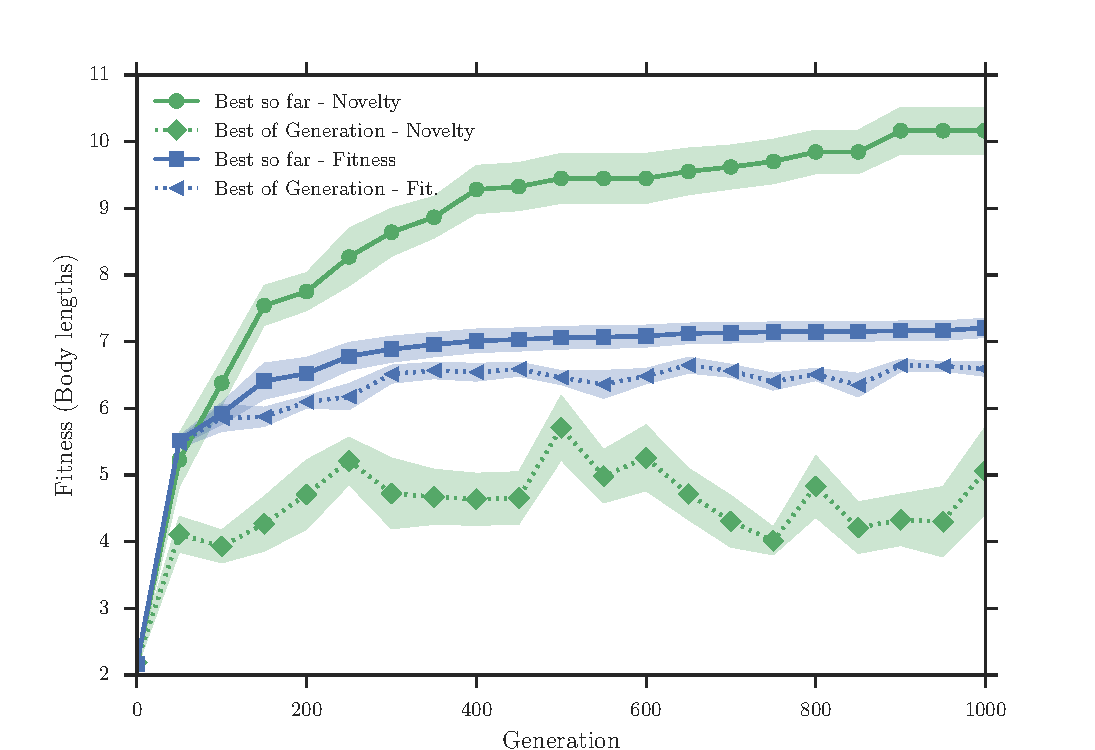
\includegraphics[width=1.0\textwidth]{../Figures/Results/AvgGenerChampNoveltyFitnessSize7.pdf}
\caption{Fitness of the generation's champion (best individual) for \emph{fitness} - \emph{novelty} search averaged over $10$ runs (settings~\ref{Settings3}).}
\label{fig:AvgGenerChampNoveltyFitnessSize7}
\end{figure}

Another aspect of the evolution should be inspected is how the population of each generation is affected in respect to the best individual per generation. In figure~\ref{fig:AvgGenerChampNoveltyFitnessSize7}, the average champion fitness of each generation is plotted over $10$ runs. Notice, that novelty search simply does not have any information about individual fitness. In fitness based search there is a clear trend that champions of each generation are getting better through the evolution resulting to an approximately increasing function. On the other hand, generations' champions in novelty search apart from the early improvement which is mainly caused by the generative encoding, follow a random pattern. What it is interesting here to see is that even though that the solutions novelty search gives, in this settings, are clearly better than the ones fitness based has, on average the champions during novelty search evolution are worse.


\begin{figure}[ht!]
\centering
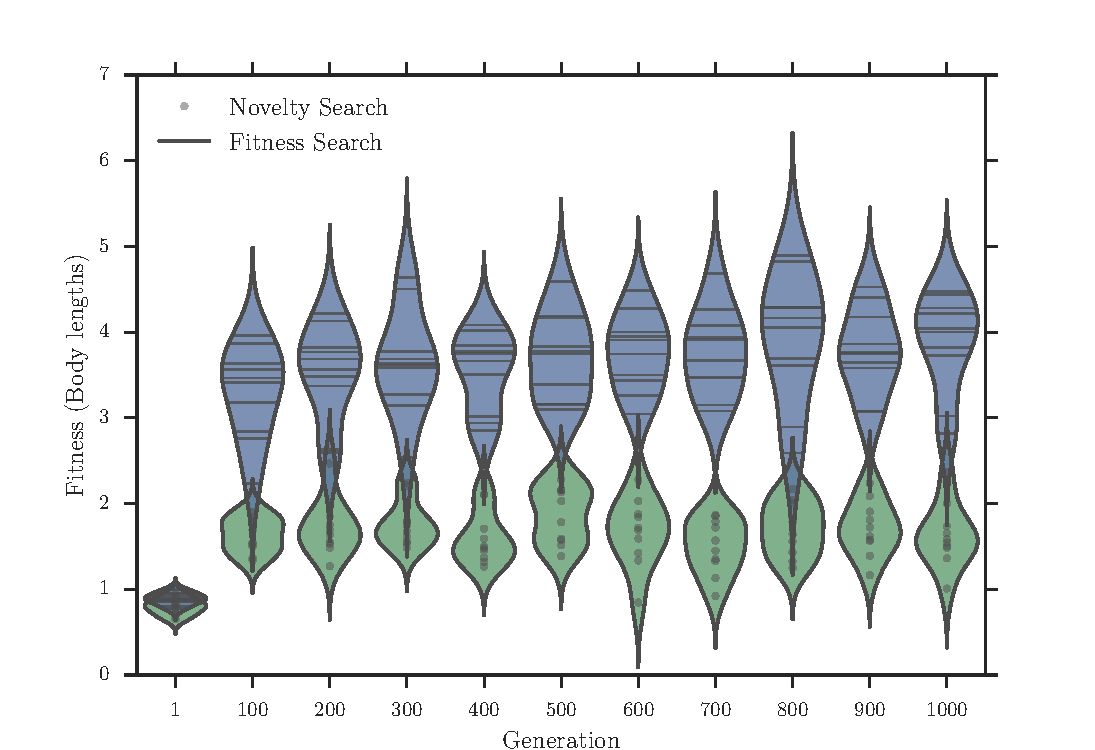
\includegraphics[width=1.0\textwidth]{../Figures/Results/ViolinPlotsAvgGenFitSize7.pdf}
\caption{Distributions of average population fitness per generation over 10 runs for \emph{fitness}(Blue) - \emph{novelty} (Green) search with generative encoding (settings~\ref{Settings3}).}
\label{fig:ViolinPlotsAvgGenFitSize7}
\end{figure}

In the same fashion, the average population fitness seems also affected by the different optimization methods. Figure~\ref{fig:ViolinPlotsAvgGenFitSize7} illustrates the distribution of population's average fitness over $10$ independent runs for \emph{novelty}-\emph{fitness} based search every $100$ generations. The resulted distributions which are shown in violin-like shapes clearly show that the average generation's fitness remains stable through the whole evolution ($1000$ generations) for both methods. What is more, the generation's average fitness is significantly lower for \emph{novelty} search, meaning that when the evolutions is being carried towards novel behavior there is no such guarantee that assumes novel new founds in the behavioral space would also be \emph{fit}.




\begin{figure}[ht!]
\centering
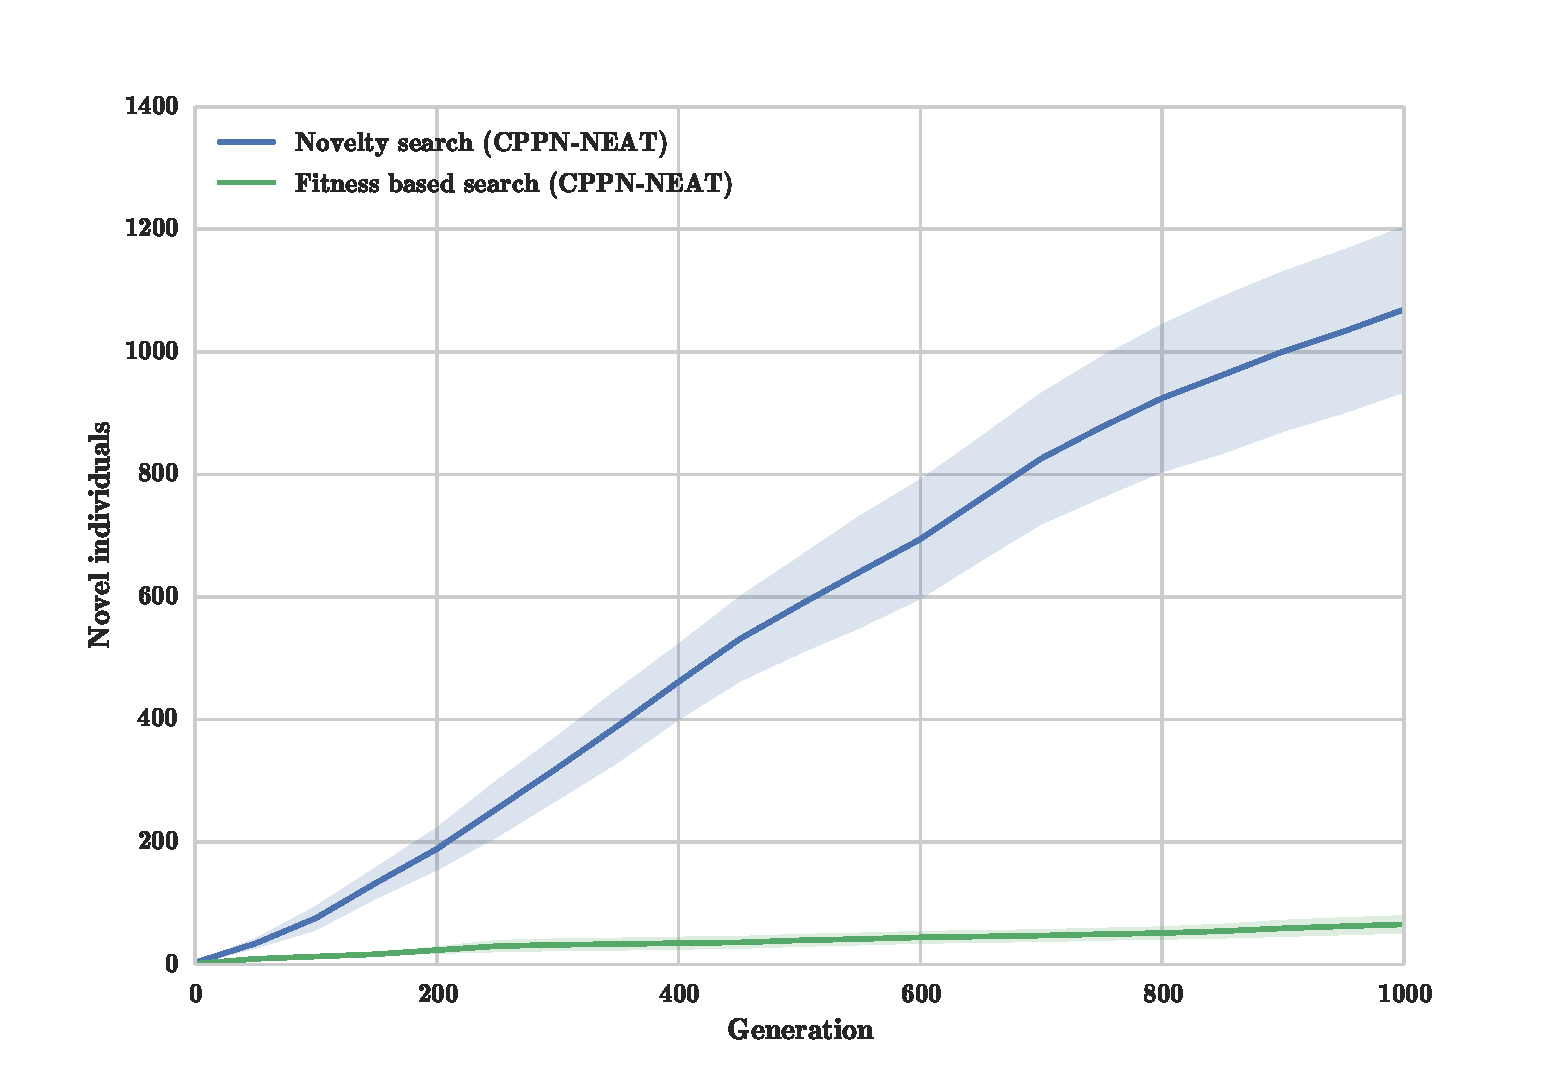
\includegraphics[width=1.0\textwidth]{../Figures/Results/novelIndividualsFitNovComp.pdf}
\caption{Number of novel behaviors up to generation number, averaged over 10 runs. The novelty measure is computed as the average distance from the $10$-nearest behaviors for \emph{fitness} - \emph{novelty} search with generative encoding (settings~\ref{Settings1}).}
\label{fig:novelIndividualsFitNovComp}
\end{figure}


Until this point, the performance in respect to an objective measure as fitness (displacement of the soft robot bodies in body lengths) has been shown. There, a method that tries to optimize genomes in respect to an objective function like fitness during the evolution is compared with a method that explicitly cares about creating diversity of the population in a behavioral level. As shown, the latter achieves to create novel individuals which are not only novel in respect to how different behaviors they have from the rest of the population they exist into, but also higher fitness than those they are optimized towards that objective. Inverting the objective function now such as our goal is to generate a wide variety of behaviors, in this case, two dimensional trajectories. Figure~\ref{fig:novelIndividualsFitNovComp}, presents the number of unique behaviors the two evolutionary methods found, averaged over $10$ runs. The resulted graph shows that comparing these two methods is pointless as \emph{novelty} search can force the evolution in going towards unvisited spaces in the behavioral space finding more novel individuals, which does not happen in normal search. Hence, \emph{novelty} achieves better results than \emph{fitness} search in both objectives set so far. 

A good behavior metric should include information about the objective function. In case of locomotion gait of soft robots a trajectory can be highly informative as far as the displacement of the robot's body is concerned. Two robot bodies which travelled the same distance into an equal time horizon, should have the same fitness if displacement only is measured, nevertheless, the locomotion strategy, is something that can only affect the actual behavior metric and not the objective function. Forcing the evolution to seek for the different in the behavior space results in finding $>10 \times$ more novel behaviors than \emph{fitness} search (depending on the threshold and the behavior metric), which  indirectly implies that high fitness individuals will be found. How the behavior metric affects the performance of the evolution is discussed in detail in the next section.



\subsection{How Behavior Selection Affects \emph{Novelty}-Search}

\begin{figure}
\centering
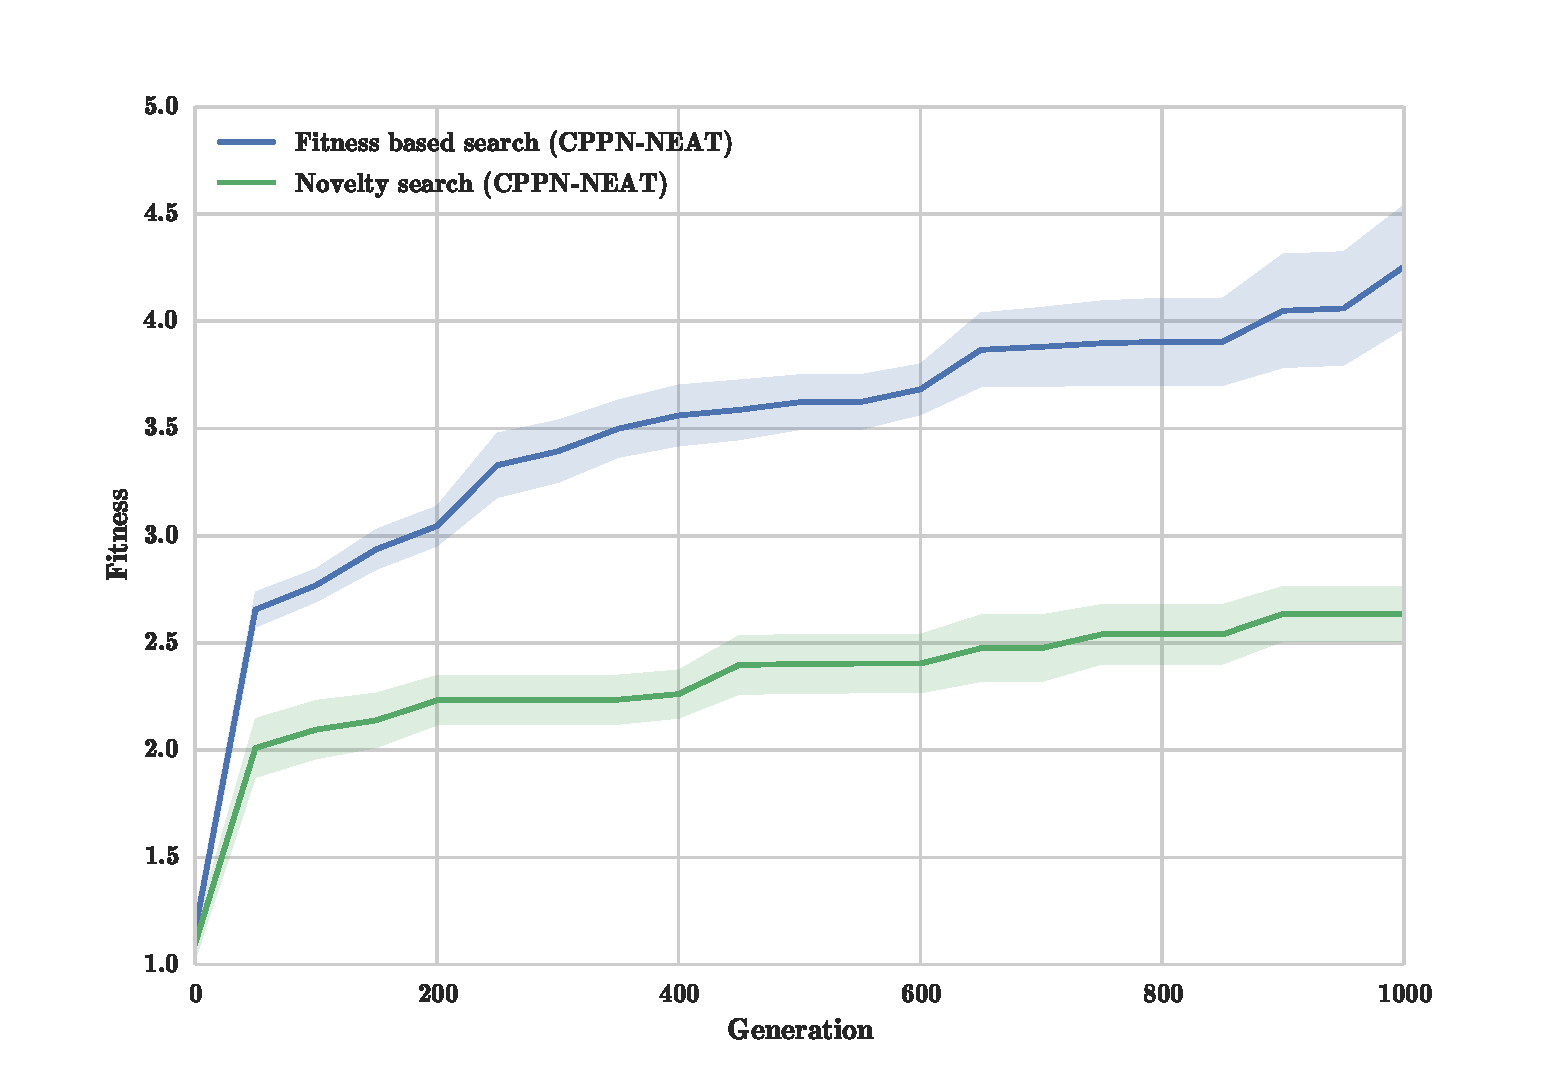
\includegraphics[width=1.0\textwidth]{../Figures/Results/FitNovSize5Pen2.pdf}
\caption[]{Best so far fitness averaged over $10$ runs, penalizing actuated materials\footnotemark for \emph{fitness} - \emph{novelty} search with generative encoding (settings~\ref{Settings1}).}
\label{fig:FitNovSize5Pen2}
\end{figure}

\footnotetext{Actuated materials penalize fitness: \[f = (1 - (n_{actuated} / n_{total})^{1.5}) \times disp \], where $n_{actuated}$, is the number of actuated voxels, $n_{total}$ total number of voxels and $disp$ the displacement of the softbot's center of mass.}


The importance of selecting a good behavior metric is important in order for novelty search to explore the behavior space to a great extent. For example searching for fast robots while you exploring the behavior space of their trajectories is a wise decision considering that all information needed to determine the fitness (speed) is incorporated inside the behavior (trajectories) assuming static sampling rate of the trajectories. In this experiment to investigate what is the result of the novelty-search evolution when no information is provided by the behavior, the behavior selected has not enough information about the actual individual fitness. The two dimensional projection of the trajectories in $x,y$-axis are again selected, while instead of evaluating the fitness in displacement, this displacement is penalized by the number of actuated voxels are inside the structure of the soft robot. Figure~\ref{fig:FitNovSize5Pen2}, illustrates the best so far fitness for both novelty and fitness search averaged on $10$ independent runs. Comparing the results with figure~\ref{fig:FitNovRandomDirectSize5}, one can notice how novelty search performs poorly in this setting. Considering that the same method outperforms traditional fitness-search evolution when the whole information of the fitness function is contained in the behavior. Trying to find novel trajectories in the first case proved successful in respect to the final displacement of the individual, from the other hand trying to maximize the distance and in the same time use few actuated voxels proved crucial for the final outcome. If the number of actuated voxels had been included in some way into the behavior, novelty-search would have been more explorative towards this direction as well.


\begin{figure}
\centering
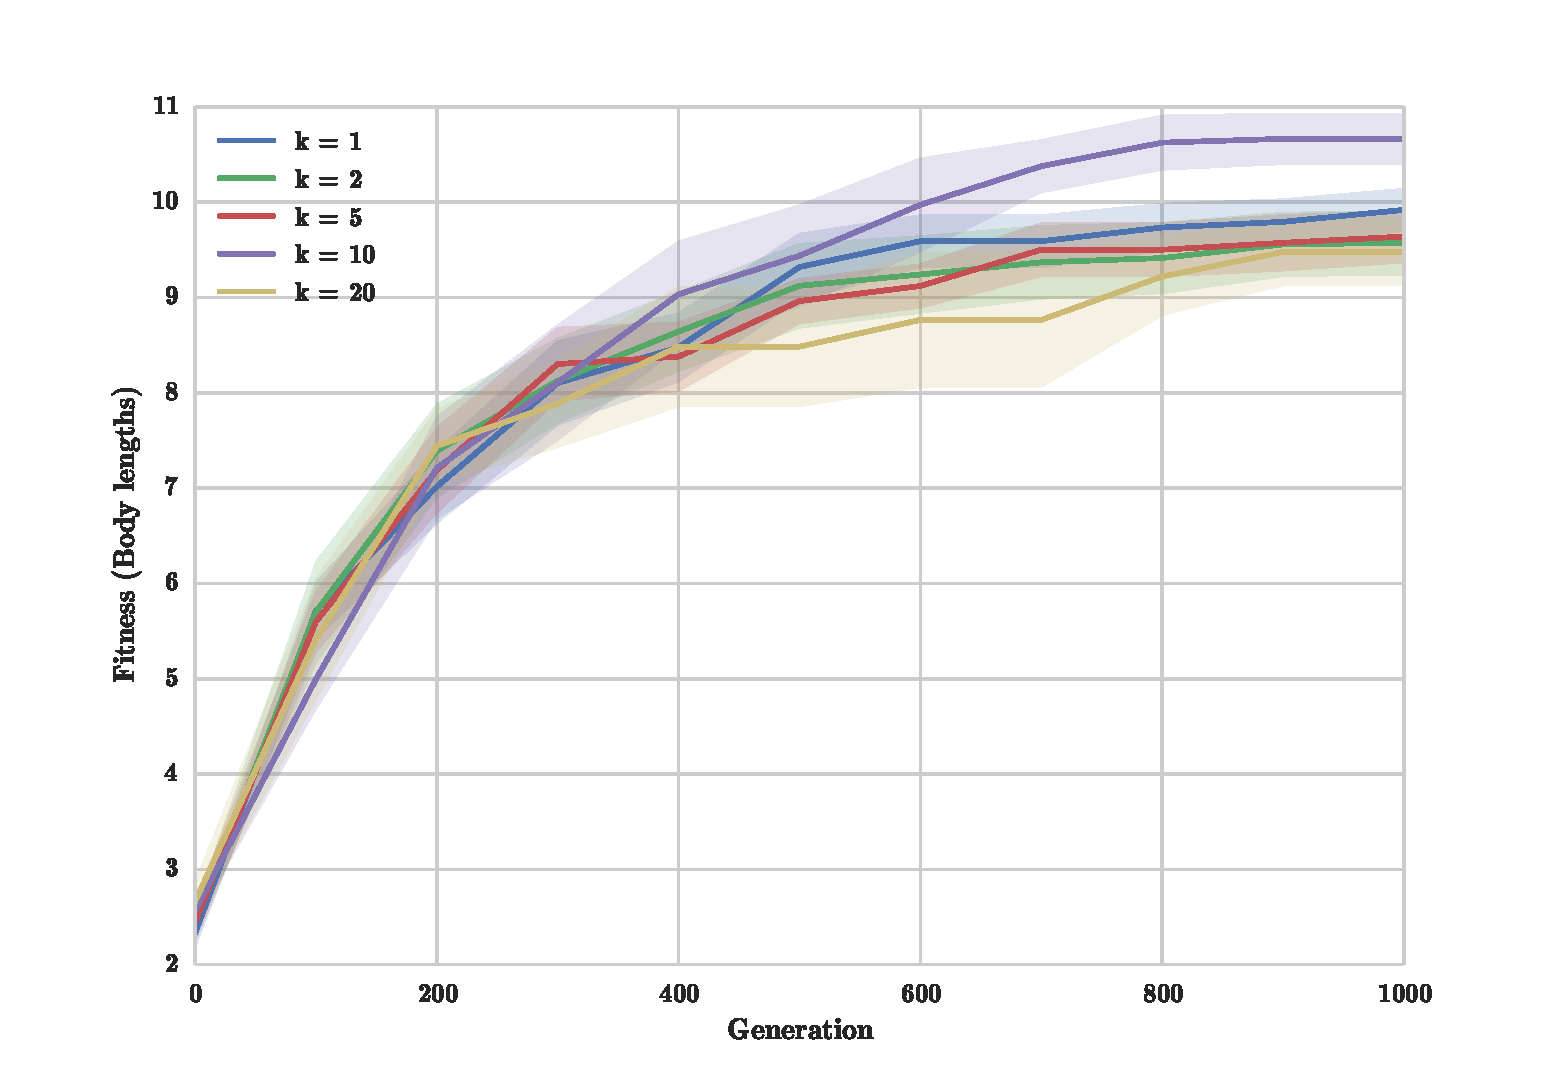
\includegraphics[width=1.0\textwidth]{../Figures/Results/KnnExperimentSize5.pdf}
\caption{Best so far fitness averaged over $10$ runs (settings~\ref{Settings1}), for different $k$ to sparsity computation of the behavior.}
\label{fig:KnnExperimentSize5}
\end{figure}

\begin{figure}
\centering
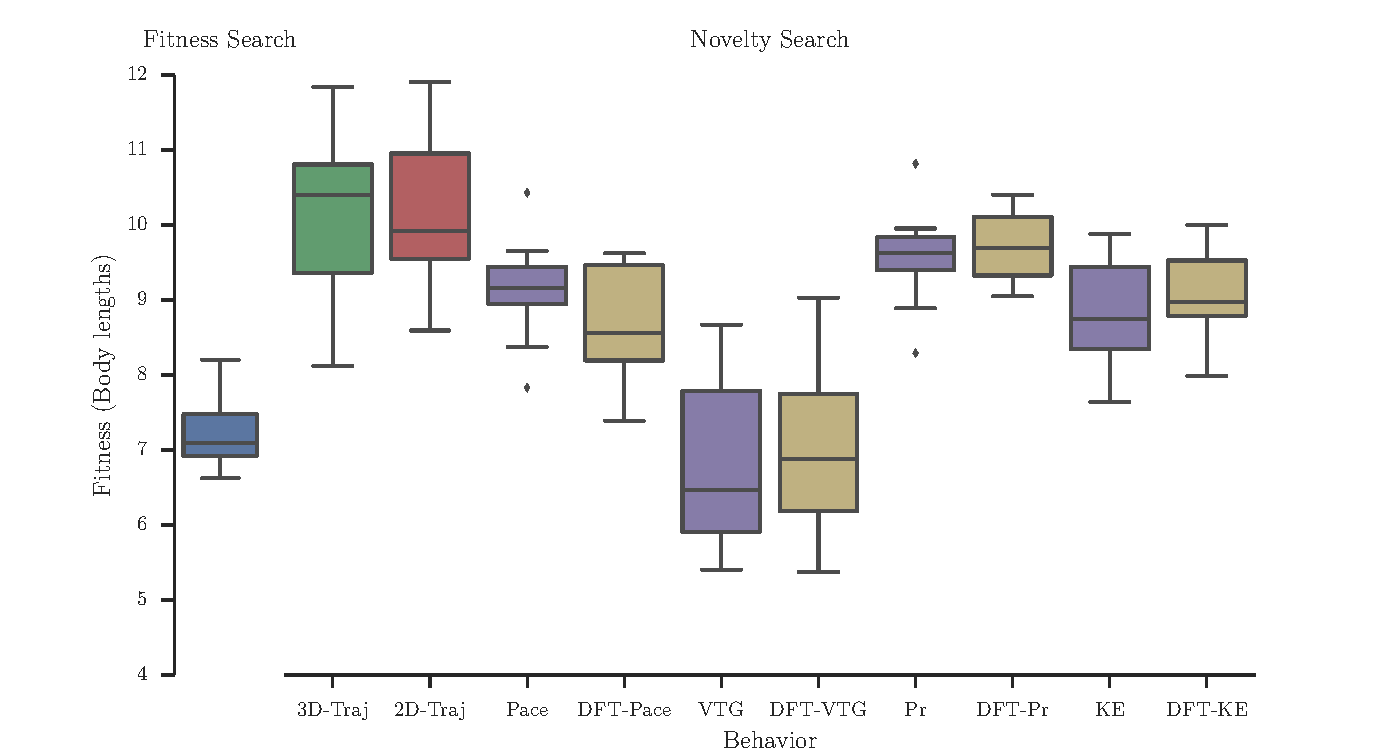
\includegraphics[width=1.0\textwidth]{../Figures/Results/BehaviorsPerformance.pdf}
\caption{Right, comparison of the evolution's best fitness result from $10$-runs under different behavioral metrics for \emph{novelty} search. \emph{Fitness} search is also evaluated under the same settings. (settings~\ref{Settings3}).}
\label{fig:BehaviorsPerformance}
\end{figure}

Sparsity (eq.~\ref{sparsenessEquation}) is the measure that defines if a newly found behavior is novel enough to enter the set of novel behaviors. Figure~\ref{fig:KnnExperimentSize5} presents the resulted best so far fitness given different values for $k \in \lbrace 1, 2, 5, 10, 20 \rbrace$. In principle $k$ can define how tolerate the algorithm can be with new behaviors. It is not certain that a specific value for $k$ should give the highest performance in fitness and it depends almost completely by the application. The only implication in choosing value for $k$ is that choosing large values should yield in a more detailed exploration in the behavior space, in the contrary using small values final set of behaviors will be denser in the behavior space. In the specific figure and experiment $k=10$ was the setting that led to the best performance.


Choosing the appropriate metric to describe a phenotype into the behavior space is crucial in the performance of novelty search. Figure~\ref{fig:BehaviorsPerformance} illustrates the experimental results under different behavior metrics, alongside the performance of pure \emph{fitness} based optimization. A set of $10$ different behavior types was used including the three dimensional trajectories of the soft robots (3D-Traj), the two dimensional projection on $x,y$-axes of the previous behavior (2D-Traj), the pace sampled every $0.001$ sec. (Pace), the discrete Fourier transformation of the same signal which was sampled every $0.00001$ sec. (DFT-Pace), the voxels touching the ground on each time-step (VTG, DFT-VTG), the maximum pressure per time-step (Pr, DFT-Pr), and the kinetic energy of the whole structure (KE, DFT-KE). What is shown here, is the fitness in body lengths of the champion individual during the whole evolution from $10$-independent runs of the experiment. Both trajectory behavior types achieve the best performance as far as fitness is concerned with a small difference in favor of the three dimensional one. Pressure is coming third achieving high performance close to the previous two trajectory behavior types, pace and kinetic energy of the structure are next in the performance ladder, and last one is the behavior signal the count how many voxels touch the ground on each time-step. The results of using $10$ different behavior types can be clustered into three performance categories. The first one which includes the two types of trajectories and achieves the best performance of all, the second one which includes raw values and the discrete Fourier transformation of pace, pressure and kinetic energy, the last and worst one with the number of voxels touching the ground. 

The performance of novelty search when trajectory of the soft bodies is used as a behavior metric is superior over all other behavior metrics. Trajectories are a very good selection for this kind of problem, since they can indirectly not only encode the objective function which is the displacement, but also the locomotion strategy and that is the reason why they explore better the landscape of behaviors resulting in such high difference in fitness against the fitness search. 

The rest of the behavior metrics apart from VTG and VTG-DFT, are close, as far as the final performance of the evolution is concerned. On reason that they fail to meet the trajectories performance is the fact that even though they keep track of features that can actually measure the performance of the robot, speed, they cannot encode the direction of the soft-body during the simulation. 

Counting the number of voxels in a structure that touch the ground in every timestep of the simulation, does not have any implication about how fast the robot is moving. A fast moving robot that is hopping can have the same behavior signature with a hopping robot that stays in the same coordinates after each jump, yet, using the trajectories these two soft-robots will have a huge difference in their behaviors.

Within the same figure and on the left side of it, \emph{fitness}-search is also evaluated under the same experimental settings. The performance of this objective optimization method is only comparable with the worst \emph{novelty}-search scenario when the VTG behavior is selected for novelty to be measured.

\subsection{Is Diversity of Individuals Increased in \emph{Novelty}-Search?}

\todo{Examples of robots here, showing that the diversity is larger for novelty}


\section{How Selection Affects the Performance of Both Search Methods}

Discussed extensively in the previous section, selection is a process that picks individuals in order to breed, be mutated or copied into the next generation. It is the part of the evolutionary algorithm that is responsible for producing the new generation, based on the individuals which exist into the current one. 


\subsubsection*{\emph{Fitness} Search}

\begin{figure}[t!]
\centering
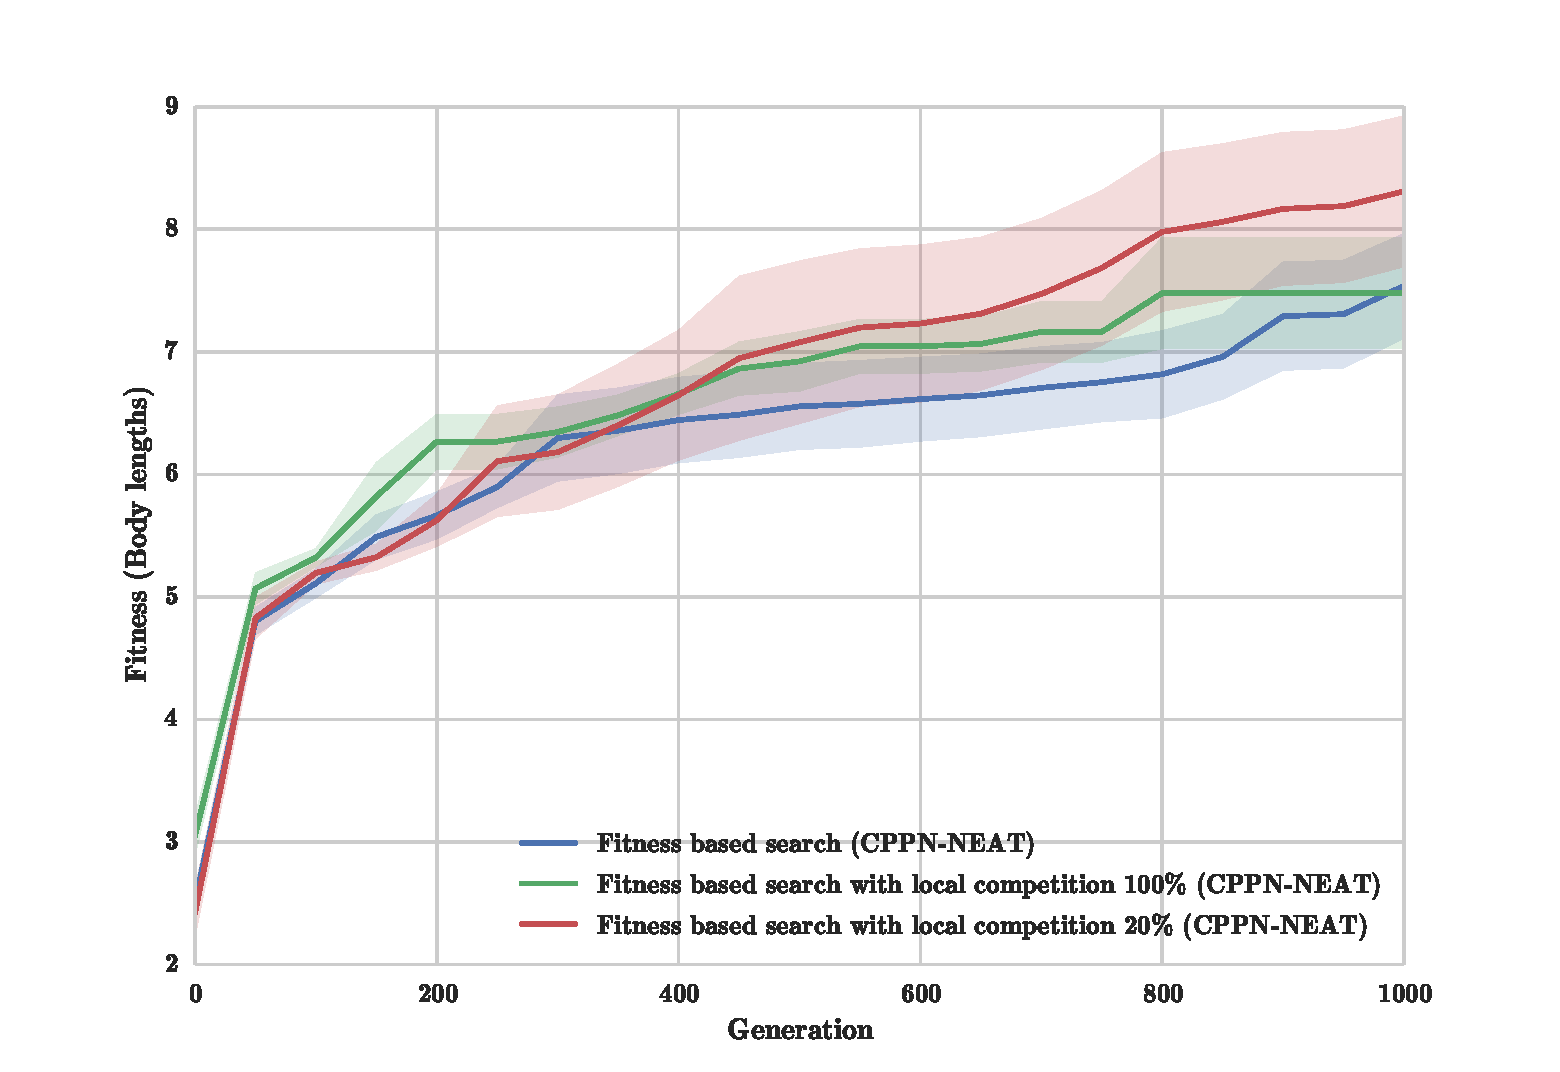
\includegraphics[width=1.0\textwidth]{../Figures/Results/fitComp100_20percent.pdf}
\caption{Best so far fitness averaged over $10$ runs, with no competition, local competition in the complete population of each species for \emph{fitness} search (settings~\ref{Settings3}).}
\label{fig:fitComp100_20percent}
\end{figure}


Figure~\ref{fig:fitComp100_20percent}, presents the results for two different selection methods, random selection from the top $20\%$ (\textcolor{MidnightBlue}{Blue}) and competition within individuals from the complete current population (\textcolor{BrickRed}{Red}). As it was expected, competition, as well as, the fact that the whole population has the opportunity to breed, contribute to the diversity of the population. This can be easily seen in this figure, random selection within the top $20\%$ of the population does not allow solution to reproduce meaning that it does not explore weaker individuals, which can later after enough mutations become better than the potential of the rest of the population. The deviation of the first method gives a perfect clue about how narrow is the fitness landscape at the converged area of search when only the best of each generation are allowed to breed.

\subsubsection*{\emph{Novelty} Search}

Since the algorithmic framework is the same for both searches, competition can be applied in novelty search as well. Figure~\ref{fig:NoveltyCompetitionsSize5}, presents the results when competition is held among individual of the whole generation's population among species in respect to different metrics. Competition is held among individual regarding their novelty among the whole population of the evolution and the novelty value they obtain if they are only compared with their species population. In both cases the overall performance of the evolution averaged on $10$ runs is worse than the default setting in novelty search where individuals to breed are selected randomly from the top-$20\%$ of the population of each species. Both selection approaches are performing poorly set side by side with the default selection method. Selecting individuals with high novelty withing the species is crucial for the performance, since these individuals can have low novel value when compared with the global population, leading to steps backwards in the evolution towards highly novel individuals. On the other hand, when individuals are competing using their global novelty measure leads to a slightly better performance, still far from the default setting, meaning that highly novel individuals can actually produce more novel individuals when they are allowed to breed.


\begin{figure}[t!]
\centering
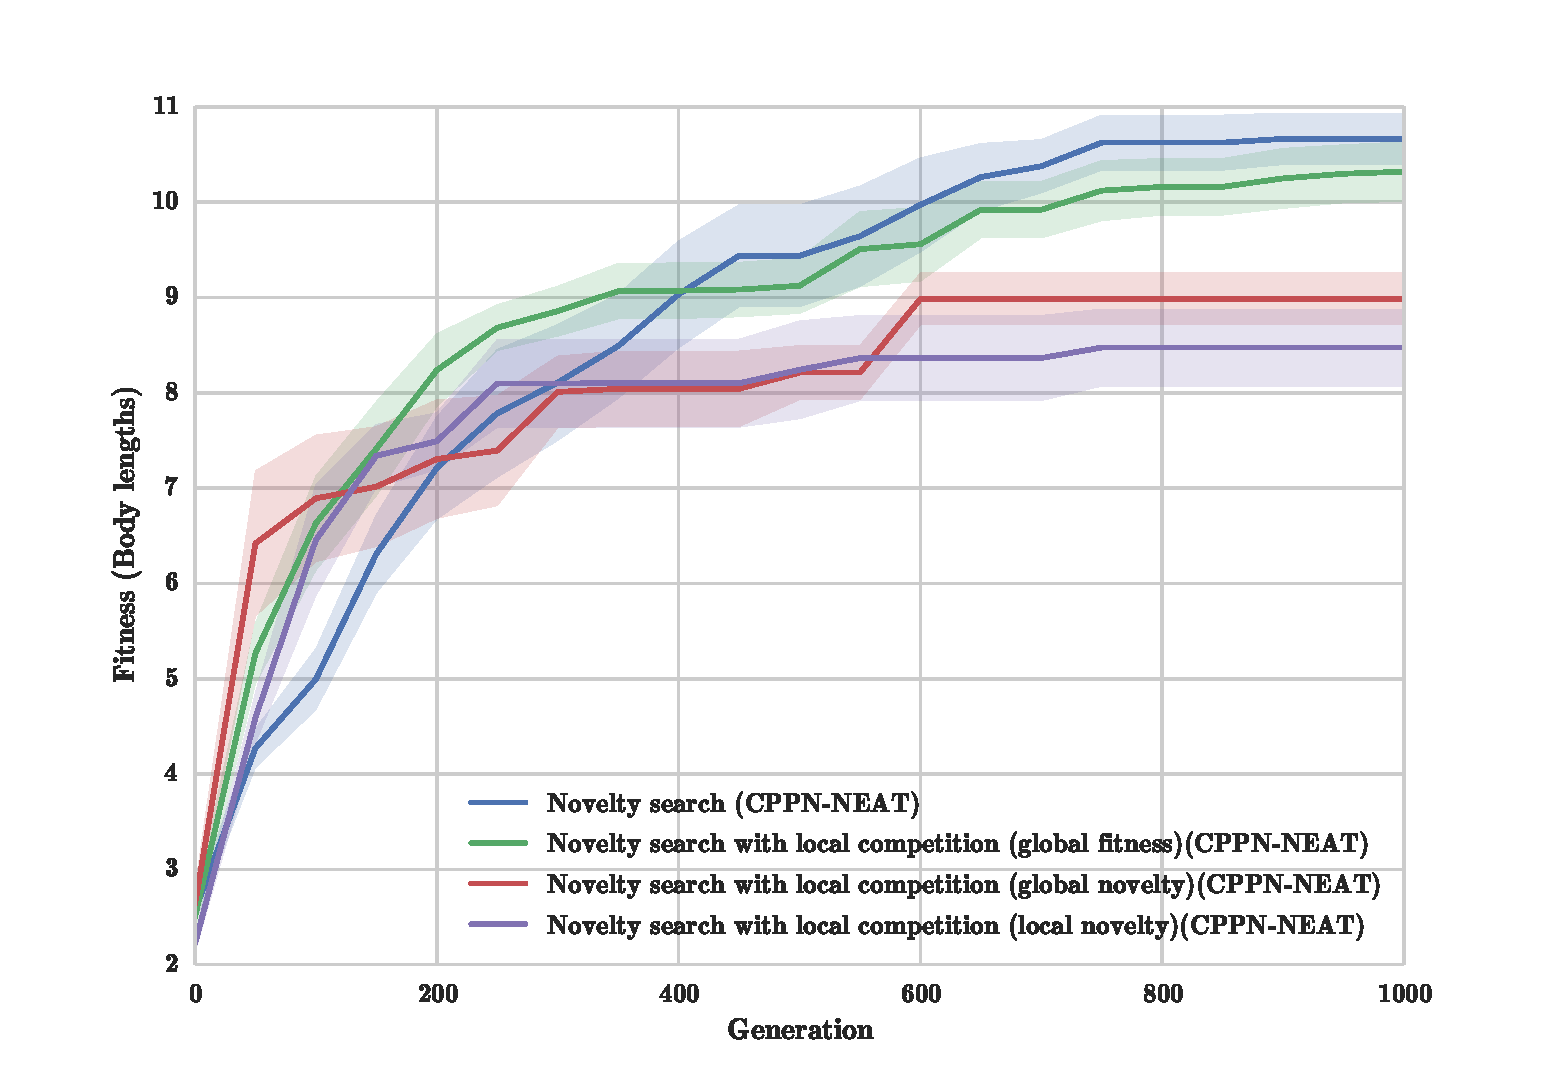
\includegraphics[width=1.0\textwidth]{../Figures/Results/NoveltyCompetitionsSize5.pdf}
\caption{Best so far fitness averaged over $10$ runs, for local competition held among the population of each species for \emph{novelty} search with generative encoding (settings~\ref{Settings1}).}
\label{fig:NoveltyCompetitionsSize5}
\end{figure}



\section{Incorporate \emph{fitness} Information into \emph{Novelty}-Search}

The reason that novelty search is considered such an revolutionary search method is because it finds solutions for deceptive problems, where the fitness landscape is not a straightforward function. What makes it so unique it is the fact that instead of looking for better solutions in respect to an objective function is looking for different solutions. In each generation of the novelty search there are some solutions that are very good regarding their objective function value, eventually these novel individuals will stop being selected for reproduction since their novelty metric value will be declined as more individuals with similar behaviors will be produced by mutations of the same novel individuals, and they won't be optimized as they could have been. Mutations and other genetic operations can optimize these fit individuals more, but this is something that happens in fitness-based search. These individuals (with high fitness values) can be seen as \emph{stepping~stones}~\cite{lehman2011abandoning} towards more optimized versions of them. Being blind to the objective function, novelty search will eventually stop producing new individuals out of them, which will lead to promising individuals being thrown out of the evolution process. 

Competition is a simple way of combining the two searches together, after each generation is produced competition is held over all the population within each specie, selecting individual, for reproduction, that have high value in the objective function. Figure~\ref{fig:NoveltyCompetitionsSize5}, illustrates the results of using the global fitness as a measure for selection among two generations. The results (\textcolor{ForestGreen}{Green} line), reveal that competition for fitness in a novelty search setting disturbs the balance of the evolution towards novelty, not allowing novelty search to expand the search in a greater extend, since it is not the case that selected fit individuals will lead in novel behaviors. 






\subsection*{Fitness Elitism in Novelty Search}

\begin{figure}[t!]
\centering
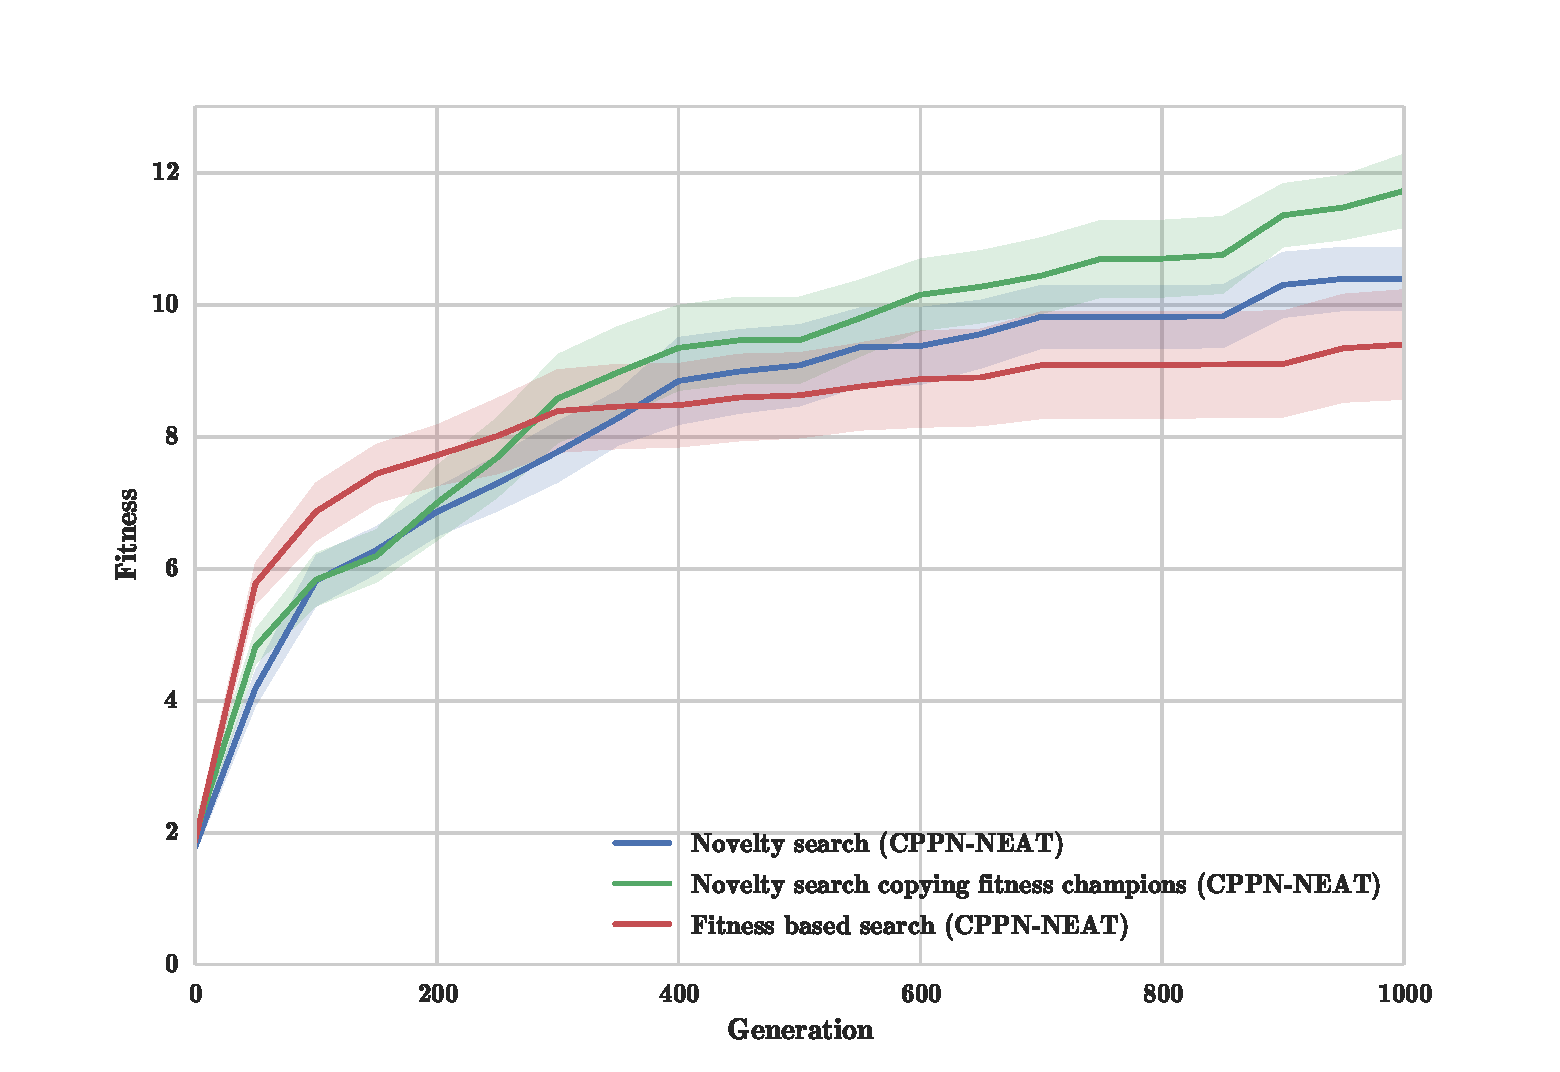
\includegraphics[width=1.0\textwidth]{../Figures/Results/CopyFitChampions10.pdf}
\caption{Best so far fitness averaged over $10$ runs, for \emph{novelty} search with and without copying \emph{fit} champions and \emph{fitness} search (settings~\ref{Settings2}).}
\label{fig:CopyFitChampions10}
\end{figure}

It is been shown, how selecting individuals in respect to their fitness distracts the evolution in novelty search. Hence, a new method is proposed for incorporating fitness information into novelty search without perturbing with its pipeline. Elitism is the process of copying the best individual of each species into the next generation with a probability of mutating it first. In this way best individuals are preserved and can be optimized later, which considered to be a successful way of protecting the best of each species generation so they can contribute with their beneficial genes later in the evolution. Novelty search can include elitism in its selection process, and it does that by copying the most novel organisms of the current population of each species to the next. Since, there is no point of changing this function, elitism can be used also to copy fit individuals within novelty search method. 

The way these two elitism functions can be used depends on the population size, and the problem. Probabilistic methods can also be used combining both elitism functions. In the specific setting, both elitism function copy new individuals to the new generations. In this way the evolution towards novelty does not get disturbed, at the same time, highly fit individuals have the chance to be optimized further as long as they are the fittest within the species population.










\section{Evolving Soft-Robots for Outer Space}



